\documentclass[11pt]{article}

\usepackage[doublespacing]{setspace}
\usepackage[margin=1in]{geometry}

\usepackage{fancyvrb}
\usepackage{cite}
\usepackage{float}
\usepackage{graphicx}
\usepackage{placeins}

\title  {``Bees?''\\ A Large Scale, Co-operative Simulation 
         Weighing Altruism and Selfishness}
\author {Alexander Simms, tRavenna Thielstrom}
\date   {CS 81: Adaptive Robotics, Spring 2014}
\begin{document}
	\maketitle

	\begin{abstract}
		% A short abstract of 200 to 300 words summarizing your findings. 

		The Prisoner’s dilemma, in philosophy, is a hypothetical situation that tests human nature. Two criminals are imprisoned. If, however, one prisoner should choose to defect and betray the other, he will be set free and the betrayed prisoner will receive 3 years of prison. If, on the other hand, they simultaneously betray each other, both will receive a 2 year sentence. Cooperative silence from both parties gets them both a lesser sentence of 1 year. Although a human may argue that altruism is the best option for both parties, game theory states that in this situation, one should always choose to betray in order to minimize personal loss, and indeed one would expect this kind of decision from an artificial agent. Yet plenty of communities exist in nature that revolve around altruistic cooperation- for example, a bee colony, where individual bees retrieve nectar for the communal hive rather than scouting selfishly for their own survival. Although cooperation can certainly be implemented into an artificial life simulation, from an evolutionary standpoint a more interesting question is raised: can the interactions of a group and the parameters of their environment produce emergent cooperation among independent agents? This research aims to investigate the possibility of emergent altruism through evolutionary game theory. To this effect, NEAT was used to evolve neural-net topologies across many generations in a bee colony simulation, testing what possible circumstances might lead to altruistic decisions or selfish decisions in the hive. Initial speculation produced a hypothesis that the amount of altruism and selfishness demonstrated in NEAT-trained agents will be most affected by an individual fitness relying on group fitness. However, the results of the experiments demonstrate that while this is partly true and group fitness is key to altering artificial behavior, in the end selfishness wins out.


	\end{abstract}

	\section{Introduction} % (fold)
	\label{sec:introduction}
		% An introduction that contrasts your study with other related work. 
		% Find and read at least three articles related to your experiment and 
		% discuss these papers here. 
		

		Cooperative behavior has frequently been discussed within the contexts of artificial intelligence. The prisoner's dilemma itself often serves as a basis for these discussions due to its relevance to issues of social order and the challenges thereof. Michael W. Macy's paper on ``Social Order in Artificial Worlds'' describes the prisoner's dilemma as the ``paradox of social order''. \cite{macy} Macy specifically names four possible outcomes in the prisoner's dilemma, ordered by the amount of payoff: temptation (defecting while the other prisoner remains silent), reward (both prisoners staying silent), punishment (both prisoners defect), and sucker (staying silent while the other prisoner betrays you). The reason why this game can be called a paradox is that the choice leading to the highest payoff (selfishness) also has the potential for the greatest failure. The experiments outlined in this paper take place not on an individual-to-individual level but rather in a large hive-type colony, they don't explicitly use the prisoner's dilemma. However, each agent has a similar choice of selfishness or altruism with somewhat similar outcomes, only on a larger communal scale. It should be noted that the experiments outlined in this paper also differ from the prisoner's dilemma in one other significant way: these experiments focus not on how selfishness in one agent causes suffering in another, but rather how selfishness negatively impacts the entire community overall, including the selfish individuals themselves.

		As mentioned by Macy, the single-iteration prisoner's dilemma is best played with a selfish dominant strategy, a conclusion that is also borne out in the experiments of this paper. However, this strategy is not the best when the prisoner's dilemma is repeated, as expanded upon in David B. Fogel's ``Evolving Behaviors in the Iterated Prisoner's Dilemma.'' \cite{fogel}  Fogel explicitly evolved best strategies over many different simulations of the scenario. A recurrent prisoner's dilemma is often effective because players will learn over time which individuals are more likely to defect or cooperate, and adjust their strategies accordingly when facing each of those individuals. However, in a hive environment where many independent agents are making the decision simultaneously, this is not a viable option to learn. Instead, for some of the experiments, recurrent networks are used to provide each generation of agents with several rounds of simulations and information from each one in order to learn general trends of the hive.

		Finally, Sarit Kraus' ``Negotiation and cooperation in multi-agent environments'' discusses the possibilities of achieving cooperation in a shared environment like the hive simulation set up for this experiment. \cite{kraus} One such strategy discussed suggests that in situations where resources must be shared, a communication system may benefit self-motivated agents. Along a similar line of thinking, Section \ref{sub:advice_from_bees} of this paper implements a system in which agents have the opportunity of increasing overall hive resources by communicating where more resources can be found. 


	% section introduction (end)

	\section{Experiments} % (fold)
	\label{sec:experiments}
		% A detailed description of your experiments. 
		% There should be enough information provided so that someone could 
		% reproduce your experiments. 

		\subsection{The Bee Model} % (fold)
		\label{sub:the_bee_model}
			To conduct these experiments, a model was developed that takes inspiration from the nectar-collecting hive insect, the bee. Our model consists of a population of individual neural nets, evolving by the NeuroEvolution of Adapting Topologies algorithm, henceforth referred to as NEAT.\cite{neat} NEAT, first developed by Kenneth O. Stanley, is a genetic algorithm that has a flexible genetic encoding that allows for the topology of the network to grow and change over time, based on a user-defined measure of ``fitness''. All of the genes within the genetic encoding are tagged with historical markings, which allows for quick implementation of ``crossing-over,'' the process by which genetic information from an individual's parents is mixed. Finally, NEAT allows for speciation: individuals within the population are grouped together based on the similarity of their genomes, and only those individuals with similar genomes are allowed to reproduce with one another. This allows for each species to find its own niche, and prevents any one species from outcompeting all of the others. It is because of these features that NEAT was selected for this task.

			Each individual NEAT agent within this model is called a ``bee'', and the population of all of the NEAT agents is called the ``hive''. Each ``day'' within this model, all of the bees leave the hive to go and find nectar. The nectar is represented in this model as a random floating-point number between 0 and 1. When it receives this nectar, it has the choice to either be selfish or altruistic. If the bee decides to be selfish, it eats the nectar then and there. If it decides to be altruistic, it brings the nectar back to the hive, where all of the nectar brought back by altruistic bees is pooled and shared equally among all of the altruistic bees. The ``fitness'' in this system is simply how much nectar a bee was able to eat on a given day.
		% subsection the_bee_model (end)

		\subsection{Basic Experiment} % (fold)
		\label{sub:basic_experiment}
			An experiment was carried out to determine the workability of the model. In this experiment, each bee lived for only one day, and afterwards died. Their fitnesses determined the makeup of the next generation of bees: the most fit bees were bred to produce hopefully more fit offspring. The NEAT network evolved with the settings described in Appendix \ref{sub:configuration_for_basic_experiment}. Its only input was the nectar it found, again, a float between 0 and 1, and output represented the choice it made. (See Figure \ref{fig:naive_system}.)

			\begin{figure}[tbph!]
				\begin{center}
					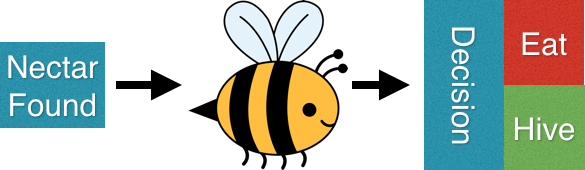
\includegraphics[scale=.5]{bee_diagrams/naive_system.png}
				\end{center}
				\caption{All that is fed into the system is the amount of nectar that the bee has found on that day, and the choice that the bee has made is determined by whether the output is closer to 0 or to 1.}
				\label{fig:naive_system}
			\end{figure}

			\begin{figure}[tbpH!]
				\begin{center}
					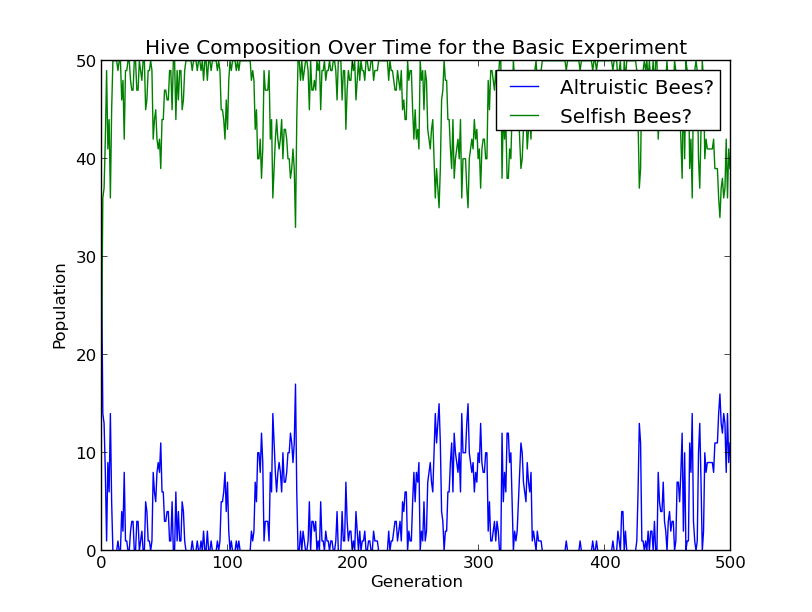
\includegraphics[scale=.5]{results/basic_comp.png}
				\end{center}
				\caption{Under the conditions of the basic experiment, altruism lost handily to selfishness.}
				\label{fig:basic_experiment_composition}
			\end{figure}

			In all of the trials run, the majority of the bees wound up selfish. A representative trial is shown in Figure \ref{fig:basic_experiment_composition}. There are a number of reasons for this, the most pressing being the fact that the bees had no direct incentive to act altruistically. While more stable fitnesses could theoretically be obtained through altruism, the system only works if a all of the bees are acting altruistically: enough bees will bring back above-average amounts of nectar to offset the bees that bring back a below-average amount of nectar. However, if too few bees are acting altruistically, then this buffering effect is not present. 


		% subsection basic_experiment (end)
		\FloatBarrier
		\subsection{Hive Fitness} % (fold)
		\label{sub:hive_fitness}
				How, then, can this selfishness be subverted? Well, in the real world, actual hives collect the	 nectar that the bees bring in, and convert it into honey. This is the inspiration for a measure of ``hive fitness,'' which is implemented as an integer between 0 and 10, indicating how much nectar the hive has on ``reserve''. Each day, when the altruistic bees bring the honey back, a tenth of the honey is taken from them and put into the hive, to support the ``queen,'' who eats 0.5 units of nectar per day. The amount of nectar in the reserve is turned into a modifier as described in Figure \ref{fig:modifier_algorithm}, which is then multiplied by the amount of nectar each bee finds to determine their fitness.

			\begin{figure}[tbh!]
				%% HERE THERE BE DRAGONS:
				%% The verbatim environment is indented with spaces because
				%% the Verbatim environment is stupid.
				\begin{Verbatim}[frame=single]
                if hive_nectar > 10:
                    modifier = 1
                elif hive_nectar > 0:
                    modifier = hive_nectar / 10
                else:
                    modifier = .00001 
				\end{Verbatim}
				\caption{The fitness of each bee is affected by the amount of nectar reserves in the hive. The modifier defined by this section of code is multiplied by the amount of nectar the bee collected in order to determine that bee's fitness.}
				\label{fig:modifier_algorithm}
			\end{figure}

			\begin{figure}[tbph!]
				\begin{center}
					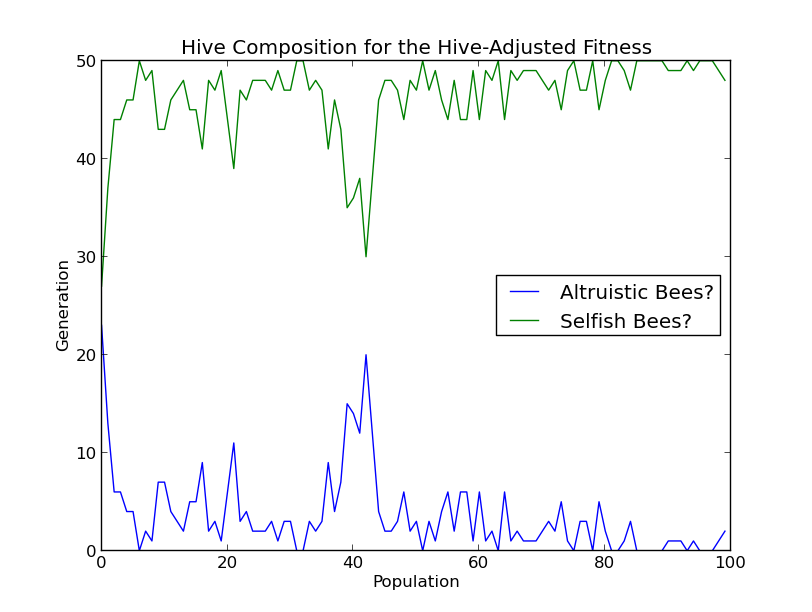
\includegraphics[scale=.5]{results/hive_fitness_comp.png}
				\end{center}
				\caption{The addition of the hive fitness component to bee fitness was unsuccessful in coercing the bees to behave more altruistically.}
				\label{fig:hive_fitness_composition}
			\end{figure}

			\begin{figure}[tbph!]
				\begin{center}
					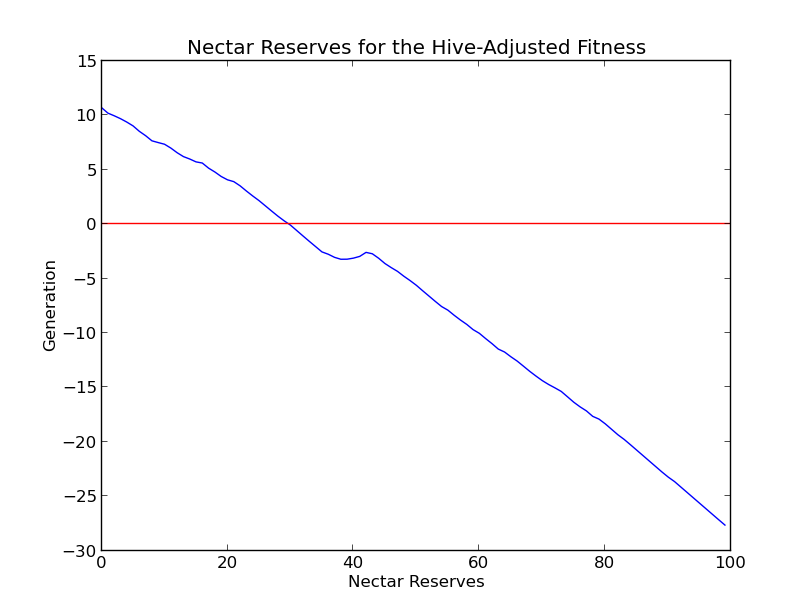
\includegraphics[scale=.5]{results/hive_fitness_res.png}
				\end{center}
				\caption{Although the bees' fitnesses continued to shrink along with the hive fitness, they did not behave altruistically.}
				\label{fig:hive_fitness_reserves}
			\end{figure}

			In this experiment, the bees still behaved overwhelmingly selfishly, for largely the same reasons as in the basic experiment. Although the hive fitness mechanic was added, the bees have no way of determining what the hive fitness currently is, and therefore have no way to adjust their actions to be altruistic or selfish, depending on the current state of the hive. Because of this, they continue to default to the same behavior of selfishness, because they are unaware of this new restriction on their behavior. Furthermore. because the same fitness modifier is applied to both the selfish bees and to the altruistic bees, the selfish bees have a similar advantage: 0.0007 is still better than 0.0001.

			Subsequent experiments were run as a proof of concept, in which the fitness adjustment was only made to the selfish bees, and in which the selfish bees were all assigned a fitness value of 0. While these produced results in which the bees all wound up altruistic, further reporting on them is outside of the scope of this paper, which is attempting to get altruism without specifically encoding for it.

		% subsection hive_fitness (end)
		\FloatBarrier
		\subsection{Recurrent Networks} % (fold)
			\label{sub:	\FloatBarrierrecurrent_networks}


			In this experiment, the bee model is considerably more fleshed-out. The bees now live for more than one day, and have considerably more inputs than they did before. Each individual day proceeds as it did in the last experiment: the bees go out to collect nectar, bring it back to the hive or eat it while they're out, and the nectar brought back to the hive is shared between the bees that brought back nectar, modulo a small amount of honey necessary to support the hive itself. However, the bees now have a way of determining how much nectar is in the hive. This is a very important input, because there fitness rests on keeping this value within appropriate ranges. 

			Recurrent networks can be much better at predicting the results that their behavior will have on their environment. Because of this, recurrent networks will used in this experiment. To get the most out of this recurrence, the bees will also have inputs corresponding to the choice they made ``yesterday,'' as well as how much fitness they got. (See Figure \ref{fig:recurrent_system})


			\begin{figure}[tbph!]
				\begin{center}
					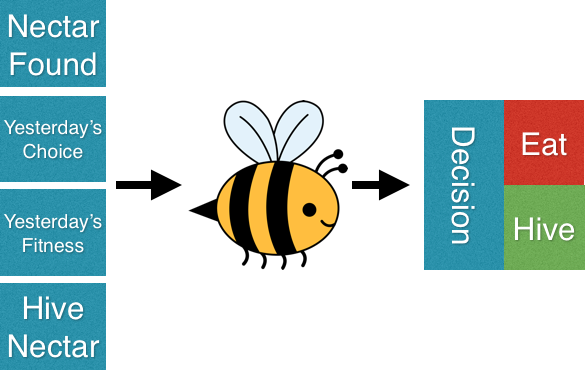
\includegraphics[scale=.5]{bee_diagrams/recurrent_system.png}
				\end{center}
				\caption{In addition to the nectar found, the networks now include the choice that the bee made yesterday, as well as the amount of fitness they received, and the level of the hive nectar.}
				\label{fig:recurrent_system}
			\end{figure}

			\begin{figure}[tbph!]
				\begin{center}
					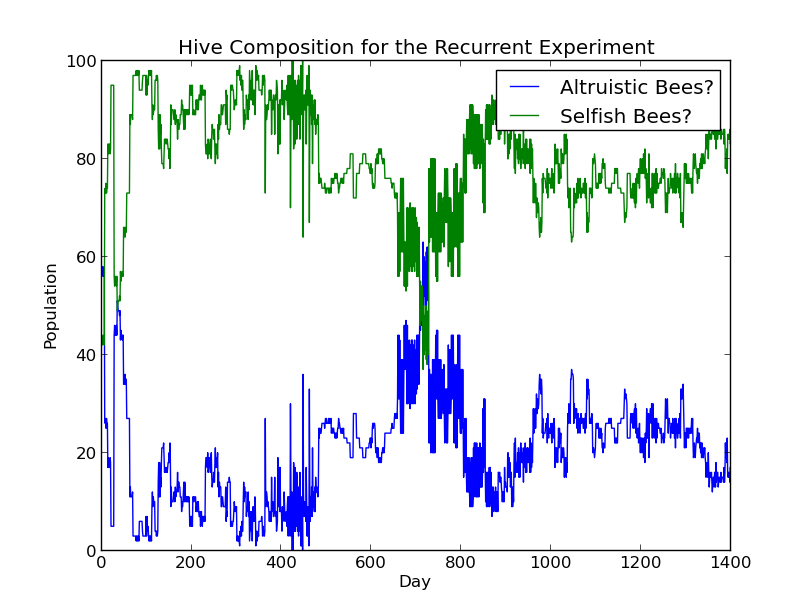
\includegraphics[scale=.5]{results/recurrent_comp.png}
				\end{center}
				\caption{The wavering pattern shown in the later generations cropped up very consistently across experiments, and serves to maintain hive nectar at a particular level.}
				\label{fig:recurrent_composition}
			\end{figure}

			\begin{figure}[tbph!]
				\begin{center}
					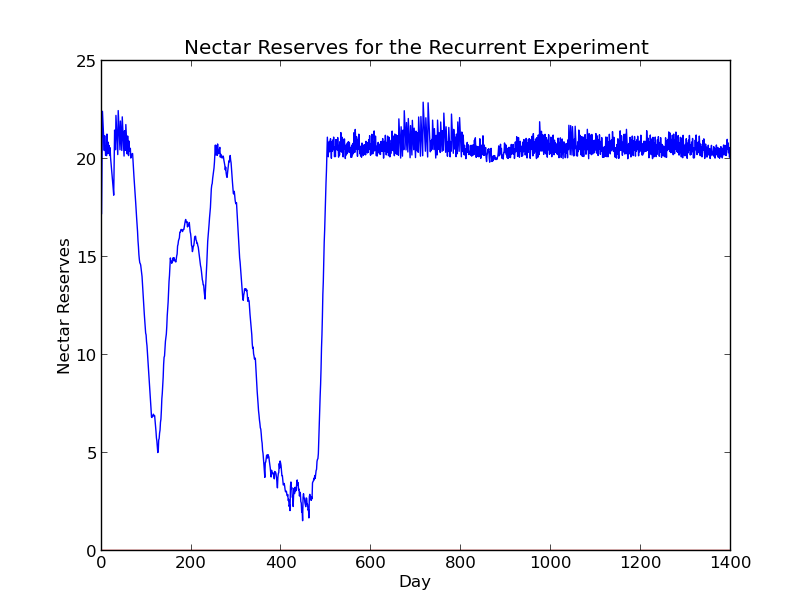
\includegraphics[scale=.5]{results/recurrent_res.png}
				\end{center}
				\caption{Under the recurrent network, the bees were able to maintain relatively high hive fitness.}
				\label{fig:recurrent_reserves}
			\end{figure}

			Under the recurrent system, consistently higher hive fitnesses were maintained (see Figure \ref{fig:recurrent_reserves}), despite the fact that the majority of the bees were selfish (see Figure \ref{fig:recurrent_composition}). This is because the bees are acting just altruistic enough to keep the hive alive, while acting selfishly for the rest of the time. This is facilitated largely by the input reminding the bees of hive nectar reserves. The nectar dips down twice in the experiment shown in Figure \ref{fig:recurrent_reserves}, however: this two drops represent the networks learning the implications of that input on their fitness. After it is discovered, they maintain the hive fitness at a reasonable level.

		% subsection recurrent_networks (end)
		\FloatBarrier
		\subsection{Advice from Bees} % (fold)
		\label{sub:advice_from_bees}

			One major factor that has been missing from this simulation of social order so far is, of course, direct interaction between the individuals. Each agent has control over their own decision, which may indirectly affect the destiny of the entire hive, but beyond this they have no opportunity to influence other members of their community, as does happen in real life. For example, another way that real biological bees cooperate within the hive is by sharing information about sites where they have foraged, essentially notifying other bees where to get the most nectar from. 

			To implement this, a second output was added to the neural network: the decision whether or not to give another bee advice. (see Figure \ref{fig:gossip_system}) This decision gets taken into account by the next bee in the population. If advice was given \emph{and} the previous bee found enough nectar for the advice to be beneficial, the current bee will take that advice and receive the same amount of found nectar as the previous bee. Otherwise, found nectar will be randomized as usual. The general aim of this experiment was to observe how the bees would choose to exploit this opportunity and what trends in altruism or selfishness might result from prosperous advice.


			\begin{figure}[tbph!]
				\begin{center}
					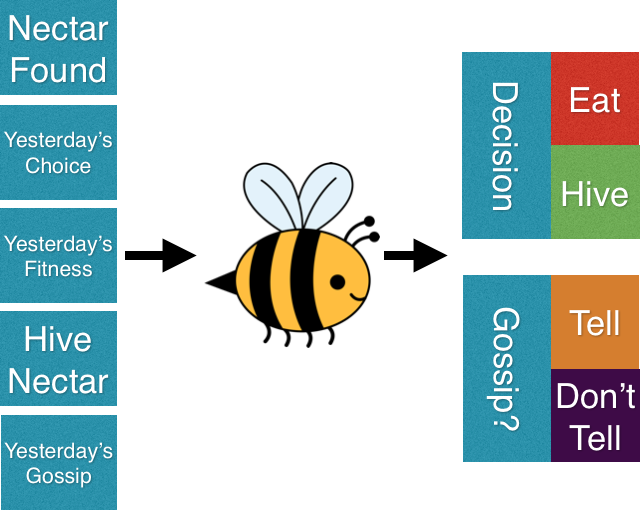
\includegraphics[scale=.5]{bee_diagrams/gossip_system.png}
				\end{center}
				\caption{In addition to the first decision output, the second output represents a choice to share helpful information with other bees.}
				\label{fig:gossip_system}
			\end{figure}

                        \begin{figure}[tbph!]
				\begin{center}
					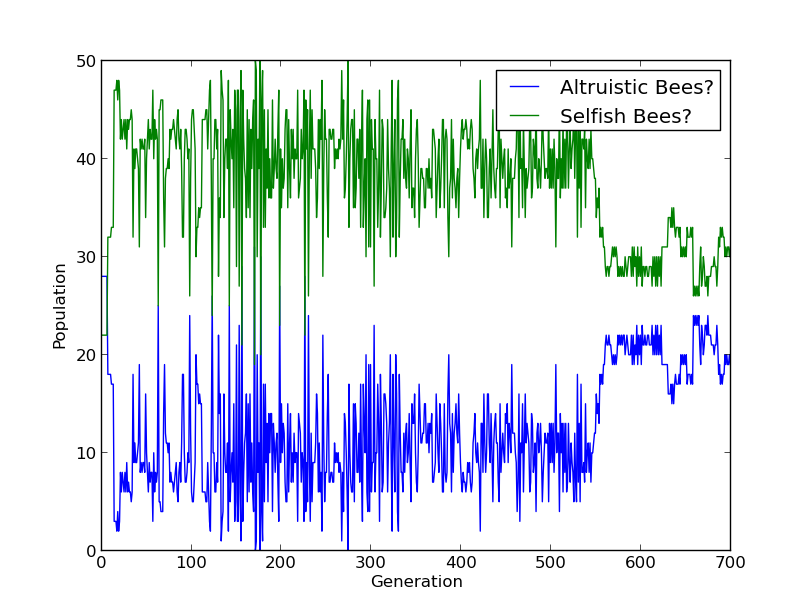
\includegraphics[scale=.5]{results/gossip_plot_twist_comp.png}
				\end{center}
				\caption{The advice system doesn't seem to generally improve upon previous experiments, but semi-positive instances certainly did occur.}
				\label{fig:gossip_composition}
			\end{figure}

			\begin{figure}[tbph!]
				\begin{center}
					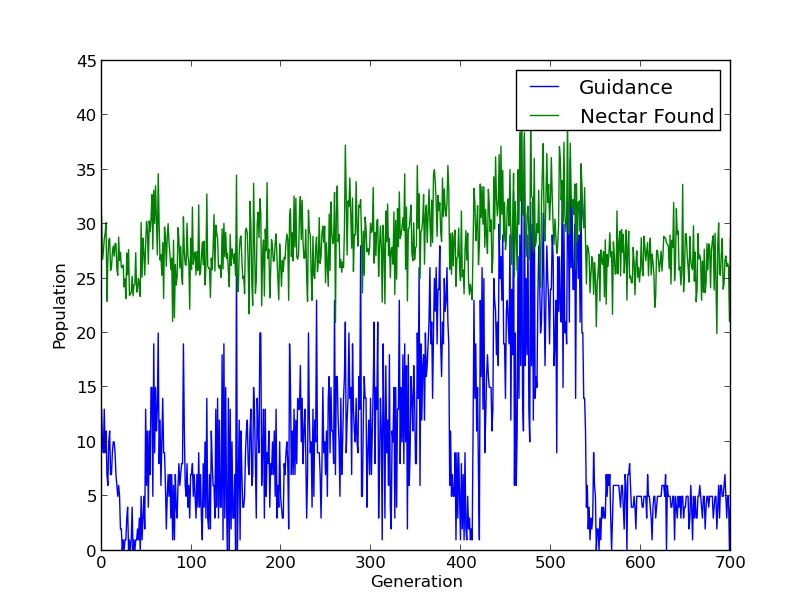
\includegraphics[scale=.5]{results/gossip_plot_twist_tell.png}
				\end{center}
                \caption{}
				\label{fig:gossip_guidance}
			\end{figure}

                        \begin{figure}[tbph!]
				\begin{center}
					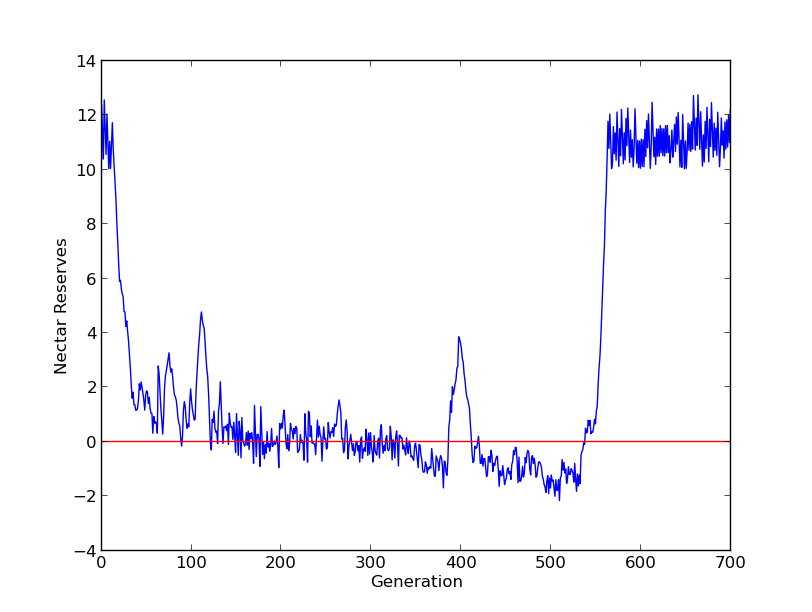
\includegraphics[scale=.5]{results/gossip_plot_twist_res.png}
				\end{center}
				\caption{An example of the negative correlation between guidance and altruism.}
				\label{fig:gossip_reserves}
			\end{figure}

			\begin{figure}[tbph!]
				\begin{center}
					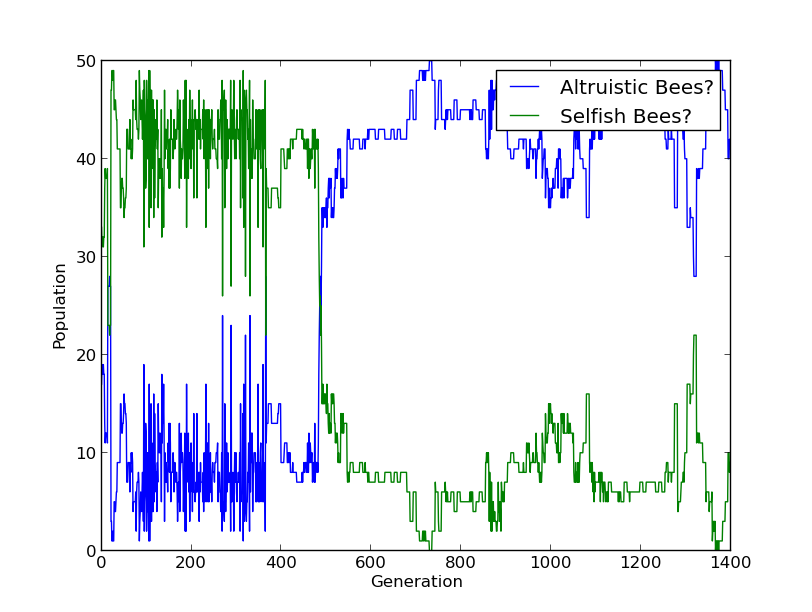
\includegraphics[scale=.5]{results/gossip_alt_comp.png}
				\end{center}
				\caption{A cooperative, altruistic society can be acheived very rarely.}
				\label{fig:altruistic_composition}
			\end{figure}

                        \begin{figure}[tbph!]
				\begin{center}
					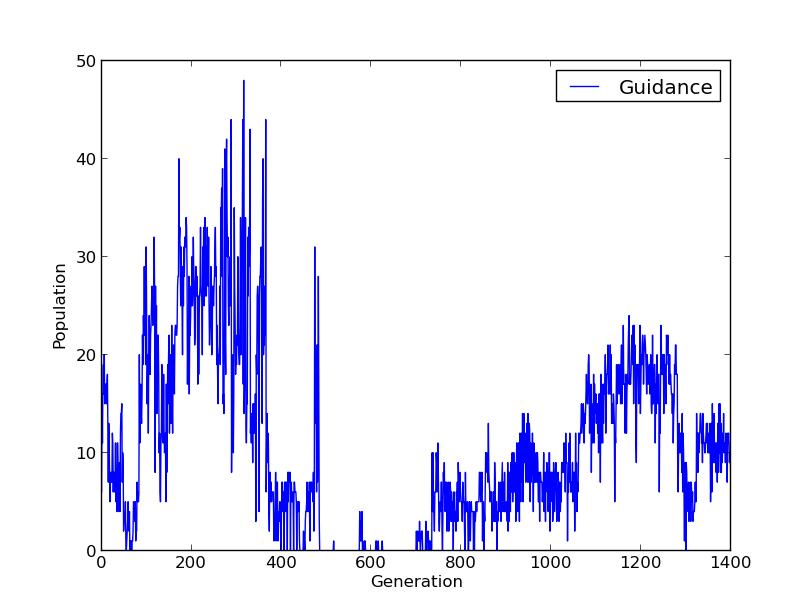
\includegraphics[scale=.5]{results/gossip_alt_tell.png}
				\end{center}
                \caption{For this to happen, it seems guidance must be first abandoned, as can be seen around the 500 day mark.}
				\label{fig:altruistic_guidance}
			\end{figure}

			\begin{figure}[tbph!]
				\begin{center}
					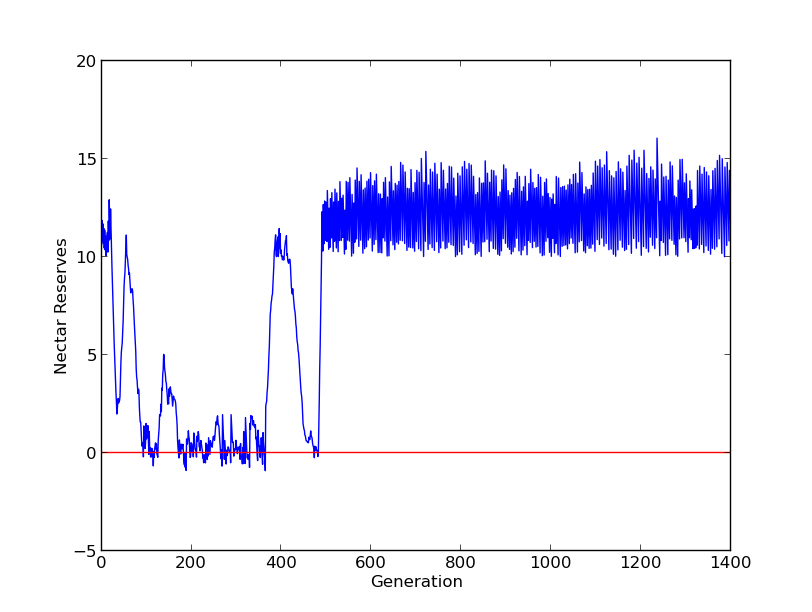
\includegraphics[scale=.5]{results/gossip_alt_res.png}
				\end{center}
                \caption{As before, there seems to be a proportional relationship between guidance and selfishness.}
				\label{fig:altruistic_reserves}
			\end{figure}


            Results from this experiment were sometimes inconclusive. Increases in guidance within the bee population generally corresponded with increases in selfishness, as seen in the Figures \ref{fig:gossip_system} - \ref{fig:altruistic_reserves} above.  However, hive fitness was affected in two different ways: some runs showed increases in hive fitness as guidance rose, and some runs showed decreases (although the latter was generally more prevalent). The rational behind this is that as guidance rises, the overall amount of found nectar rises, so hive fitness is more likely to rise if there are an acceptable amount of altruistic bees. On the other hand, bees that are consistently receiving an above average amount of nectar through guidance are also more likely to behave selfishly instead of altruistically, which obviously will decrease hive nectar. Overall, it seems that a lack of guidance actually corresponds to higher amounts of altruism, although to understand why this might be the case further research would be necessary. The system of one-way communication implemented here, then, seems to achieve the opposite of the desired affect. Yet, this was also the only experiment for which actual altruistic evolutions were found, despite having a very low frequency of appearance in our various experimental runs. Experiments under the exact same conditions and parameters were also repeatedly run without the advice system, but clear altruism was never exhibited. This would seem to suggest that the presence of the advice system is necessary somehow to achieve even these very rare results.
		% subsection advice_from_bees (end)

	% section experiments (end)
	\FloatBarrier

	\section{Discussion} % (fold)
	\label{sec:discussion}

		As has been demonstrated, is rather difficult to get independent agents to achieve altruism in this sort of environment. It has been theorized that actual bees have some sort of urge hard-coded into their genetics to be altruistic, and this is how hives are able to survive. \cite{macy}

		One substantial difficulty for the development of altruism in our particular model comes from the way that the fitness function is implemented. All of the bees coming back are coming back with nectar in the range of 0 and 1, so amortized, choosing to be altruistic is choosing a fitness of $0.5$. Choosing to be selfish has the potential to obtain much higher fitnesses than that, and those individuals will be able to reproduce, at the cost of the altruistic individuals of the hive.

		It is important to note that altruism is of course perfectly possible and easily implemented, as has been mentioned in Section \ref{sub:hive_fitness}, along with other test runs in which each bee's fitness was simply the overall hive fitness. If the programmer explicitly rewards or punishes behaviors, or directly links motivation solely to the group rather than the individual, good results can be achieved, but at the cost of the factor of self-motivation and inherent self-interest that is present in real life communities. Despite the nature of this experiment, a hive mind is undesirable. Although our results are not as promising or as optimistic as initially hoped for, further research on self-motivated independent cooperation would be valuable. 

		%for comparison to Macy
		\begin{itemize}
		\item Temptation: selfish agents receive a random (potentially above average) fitness
		\item Reward: altruistic agents receive an average fitness
		\item Punishment: enough agents are selfish that hive fitness drops for all
		\item Sucker: a minority of agents behave altruistically while a majority behave selfishly, reducing hive fitness for all
		\end{itemize}
		Unlike the true prisoner's dilemma, instead of temptation/sucker and reward/punishment being linked, our experiment has temptation/reward and punishment/sucker linked. Also, punishment and sucker potentially receive the same amount of low payoff. This could supposedly lower the potential for selfishness since acting altruistically no longer possibly leads to a worse ending than acting selfishly.

	% section discussion (end)


	\nocite{*}
	\bibliography{bib}
	\bibliographystyle{plain}

\end{document}
